\documentclass{article}
\usepackage[utf8]{inputenc}
\usepackage{url,graphicx,tabularx,array}
\usepackage{amssymb}
\usepackage{mathtools}
\usepackage{amsmath}
\usepackage{enumerate}
\setcounter{secnumdepth}{5}
%\usepackage{fullpage}
\usepackage[margin=1in]{geometry}
\usepackage{multicol}


\begin{document}


\pagenumbering{gobble}


\begin{multicols}{2}
\section{Introduction}
Mushroom edibility is determined by lots of different attributes. Conducting a poison test every time before eating is not realistic. Therefore, a method that enables us to judge the edibility by looking at its physical properties like color, shape, habitat etc., is essential. In this study, we use classification methods to develop a rule for differentiating edible mushrooms from poisonous ones. The dataset includes hypothetical samples corresponding to 23 species of gilled mushrooms in the Agaricus and Lepiota Family with 8124 instances and 22 attributes. We noticed 2480 missing values in the “Stalk Root” attribute, and after further investigation, we found out that they were not missing completely at random. Therefore, we decided to treat the missing values as another category of this attribute. 

\section{Machine Learning Method}
Due to the categorical nature of data, the number of classification algorithms available is rather limited. Eventually, we chose the \textbf{naive Bayes classifier} as the one to work with. In general, Bayesian classifiers assign the most likely class to a given instance described by its feature vector, and naive Bayes imposes a strong (naive) assumption that features are independent given class. Given feature variables $F_1,...,F_n$, a Bayesian classifier aims at computing the probability
\begin{align*}
p(C\vert F_1,...,F_n)
\end{align*}
where $C$ denotes a class variable with some number of classes.\\

Using Bayes' theorem, we have:
\begin{align*}
p(C\vert F_1,...,F_n) &= \dfrac{p(C)p(F_1,...,F_n\vert C)}{p(F_1,...,F_n)}\\
&\propto p(C,F_1,...,F_n)
\end{align*}
Using the chain rule on the right-hand side, it follows that:
\begin{align*}
p(C\vert F_1,...,F_n) \propto p(C)p(F_1\vert C)p(F_2\vert C,F_1)\\
\dotsb p(F_n\vert C,F_1,...,F_{n-1})
\end{align*}
Since $F_k$'s are mutually independent conditioning on class $C$, the joint model above becomes:
\begin{align*}
p(C\vert F_1,...,F_n) \propto p(C)\prod\limits_{i=1}^n p(F_i\vert C)
\end{align*}
and the exact value of the prediction probability is then:
\begin{align*}
p(C\vert F_1,...,F_n) = \dfrac{1}{Z} p(C)\prod\limits_{i=1}^n p(F_i\vert C)
\end{align*}
where $Z=p(F_1,...,F_n)$ is free from class $C$ and only depends on values of the feature vector.\\

The class prior $p(C)$ and feature probability distribution $p(F_i\vert C)$ can be approximated from the training set. A class prior can be calculated by assuming equiprobable classes, or directly estimated by relative frequencies in the sample. The approximation of the feature distribution, however, requires us to impose a distribution on the features in the training set. In this study, each feature is either a binary or multi-class categorical variable. Therefore, the Bernoulli (for binary) and multinomial (for multi-class) distributions are natural choices for feature distribution.\\

After prediction probabilities are acquired, a classification rule is needed to assign class labels to new instances. Sometimes, the \textit{maximum a posteriori} (MAP) decision rule is used, in which an instance is placed in the most probable group. However, when the problem is a binary classification, a threshold is often used to determine the class label: if the prediction probability falls above the threshold, the instance is labelled positive, and if not, negative.\\

To assess the performance of this classifier in practice, we applied a $K$-fold cross validation: the data set is split into six equally-sized subsets and we applied naive Bayes six times, each time leaving out a different subset to be tested while using the remaining five as the training set. At first, we used the \textit{Receiver Operating Characteristics} (ROC) curve to select an optimal threshold to map instances to predicted classes. Then we constructed confusion matrices and computed the \textit{Apparent Error Rate} (APER), defined as the fraction of misclassified sample observations, for each run of cross validation as well as their average. Finally, we calculated the \textit{False Negative} (FN) rate for each run, which, in this study, is defined as the probability of classifying a poisonous (positive) mushroom as being edible (negative), because this situation leads to more deadly consequences than getting a false positive and hence is our major concern.





\section{Findings}
\subsection{ROC Curve}
A ROC graph is a technique for visualizing and selecting classifiers based on their performance (Fawcett, 2005). In this study, we use it to select the optimal threshold for prediction probabilities. ROC curves are two-dimensional graphs in which true positive (TP) rate is plotted against false positive (FP) rate. An ROC graph depicts relative tradeoffs between benefits (TP) and costs (FP). Ideally, an optimal classifier is one that identifies all true positives and no false positives. Therefore, roughly speaking, the more "northwest" a point lies in ROC space, the better the corresponding classifier performs.\\

For a probabilistic classifier such as naive Bayes, each point in ROC space corresponds to a different choice of threshold. We constructed a ROC curve for each fold of cross validation and averaged the curves at each threshold. The resulting graph is as follows:
\begin{center}
  \scalebox{0.28}{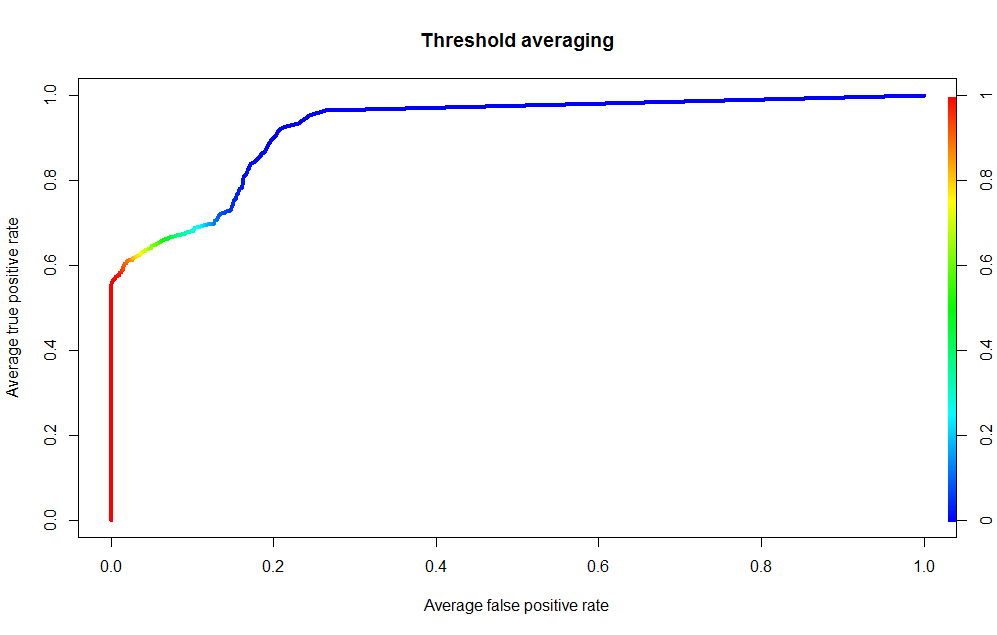
\includegraphics{fig/avg_ROC.png}}
\end{center}

Notice that according to the color palette, the upper left corner corresponds to threshold values close to zero.

\subsection{APER and False Negative Rate}
Based on the ROC plot above, we set the threshold to 0.005, which is close to zero. Using this classification rule, the APER and FN rate of each run are as follows:\\

\begin{center}
\begin{tabular}{|c|c|c|}
\hline
\textbf{Run} & \textbf{APER} & \textbf{FNR}\\
\hline
1 & 0.0798 & 0.0392\\\hline
2 & 0.0214 & 0.2302\\\hline
3 & 0.0805 & 0.2013\\\hline
4 & 0.0517 & 0.0234\\\hline
5 & 0.0805 & 0.0428\\\hline
6 & 0.2349 & 0.0385\\\hline\hline
\textbf{avg} & 0.0798 & 0.0392\\
\hline
\end{tabular}
\end{center}
%\caption{APER and FNR for each run and their averages}
%\end{table}

Therefore, on average, with our choice of threshold, the naive Bayes classifier mistakenly classifies $7.98\%$ of mushrooms, and $3.92\%$ of poisonous mushrooms are wrongfully identified as being edible.






\section{Discussion}
\subsection{Assumptions}
As we mentioned in Section 2, the main assumption of naive Bayes is independence between features given class labels. Although this assumption is unrealistic in practice, it has been shown that naive Bayes may still have high accuracy on datasets in which strong dependencies exist among attributes (Zhang, 2004). The reason behind the classifier's robustness remains an open question.
\subsection{Scaling to Big Data}
The dataset we worked with contains 8124 observations and 22 independent variables. The actual running time of the six-fold cross validation is 6.13 seconds, and we expect this time to increase at least linearly with sample size. Suppose a new categorical variable with $k$ levels is added, then if we assume a multinomial distribution, an extra $k-1$ parameters need to be estimated. 







\begin{thebibliography}{}

\bibitem{}
	Fawcett, T. (2005):
	"An introduction to ROC analysis",
	\textit{Pattern Recognition Letters}, 27, 861-874  
  
\bibitem{}
	Zhang, H. (2004):
	"The optimality of naive Bayes",
	FLAIRS2004 conference
	
	
\end{thebibliography}


\end{multicols}


\end{document}